
\subsection{Sequence Diagram Use Case 2}

I sekvensdiagrammet nedenfor beskrives den overordnede interaktion mellem systemets dele i konteksten af Use Case 2. Systemet initierer udrugningssekvensen, hvor der kontinuert reguleres på temperatur og luftfugtighed, og hvor der tjekkes om æggene skal vendes. Når denne sekvens er afsluttet, informerer systemet brugeren om dette. Dernæst reguleres temperatur og luftluftighed indtil alle udrugede emner er fjernet fra systemet. Herefter stoppes regulering af temperatur samt luftfugtighed, og systemet går i sin idle-state.

\begin{figure}[H]
\centering
\includegraphics[page=2,width=\linewidth,viewport=8mm 265mm 268mm 573mm]{./2_systemarkitektur/diagrammer/ArkitekturDiagrammer.pdf}
\caption[Diagram]{Sequence diagram - Use Case 2}
\label{fig:SystemStateDiagram}
\end{figure}
\clearpage
